\documentclass[a4paperpaper,twocolumn]{article}
\usepackage{lmodern}
\usepackage{amssymb,amsmath}
\usepackage{ifxetex,ifluatex}
\usepackage[T1]{fontenc}
\usepackage[utf8]{inputenc}
\usepackage[unicode=true]{hyperref}
\usepackage{graphicx}
\usepackage{authblk}
\usepackage{eso-pic,lipsum}
% Massively reduces whitespace.
\usepackage{savetrees}
% For tables.
\usepackage{booktabs}
\setlength{\heavyrulewidth}{1pt}
\setlength{\abovetopsep}{3pt}
% For referencing.
\usepackage[backend=biber]{biblatex}
\addbibresource{write_up.bib}

\begin{document}
\title{\huge \\Latent Dimensionality Reduction: An Algorithmic Method for Interpreting Black Box Models\\~\\
\Large \emph{DRAFT - TENTATIVE}}
\author{\emph{Elias Kassell, Fred Farrell}}
\date{TODO 2019}
\maketitle

\section{Abstract}\label{abstract}

LDR (Latent Dimensionality Reduction) allows users to interpret any model by decomposing predictions in a high dimensional space into a lower dimensional space, eliminating the requirement for feature reduction prior to model training. Both the output of the model and the certainty of its predictions are encoded in the condensed space. This dimensionality reduction is done by approximating the model's prediction as a function, drawing samples using the VEGAS algorithm, interpreting the space using Monte Carlo Integration, then using either binning or an ensuing model to estimate prediction certainty. This ability to glimpse higher dimensional spaces, which are normally too complex for humans to understand, represents a powerful tool in improving the underlying features generating the metrics.

\section*{Acknowledgements}

TODO

\section{Introduction}\label{Introduction}

Black box models are notoriously difficult to interpret. This makes them impractical for situations where it is a necessity to understand why a model has chosen a particular output as its prediction, and what effect changes to values of the input features will have on the output of the model.

Some of the real world implications that interpreting black box models provides include

\begin{enumerate}
\item Interpreting how the value of a feature, or subset of features, affects a model's prediction, which henceforth is referred to as "feature interpretation". For example, in a medical setting this interpretation can be used for suggesting the relation between features and a diagnosis. In another example, in manufacturing this interpretation can provide target values for the underlying processes involved in quality of produce.

\item The ability to use a model when not all values for the input features are present. By integrating across features which are not present, the certainty of a models prediction can be estimated. Current methods, such as imputing values for features which are not present, ignores the variability of the absent features across the feature space, which LDR provides.
\end{enumerate}

\section{The Algorithm}

\begin{enumerate}
\item Normalize the original data so it falls into [0, 1] intervals.
\item Train a predicting model on the normalized data.
\item Train a OCSVM (One Class Support Vector Machine) [OCSVM], or an alternative model for detecting outliers, on the normalized data.
\item Create a KDE (kernel density estimate) [KDE] of the training points with a bandwidth equal to some resoltuion $r$. If the original model is a classification, create equal density across all classes (can be done by duplciating points).
\item Sample $n$ new points from the kernel density, using both classifiers to make predictions of each point. Weight the prediction according to the outlier classifier, where outliers have no model certainty in the prediction at that point.
\item Two options are available here, where single feature interpretation is easiest done with binning, while with multiple feature interpretation it is more sensible to use a regression SVM (support vector machine) [] or alternative function descriptor.
    \begin{enumerate}
        \item Binning: for each dimension, group points with resolution $r$, reducing the value of the bin to the mean prediction across it.
        \item SVM: for each dimension, train a regression SVM to estimate the prediction across the feature space. Use the SVM to make predictions across the space with double resolution, $r \times 2$.
    \end{enumerate}
\end{enumerate}

\section{Classification Example}

The Wisonsin breast cancer dataset is used as it has 31 dimensions. The aim with the dataset is to classify the tumor as either malignant or benign. There are 569 samples in total, with 357 benign and 212 malignant.

\subsection{Random Forest and OCSVM Interpolation}

The 100 estimator RF (Random Forest) achieved an F1 score of 0.975, while the OCSVM was trained to interpret 10\% of training values as outliers. Benign was selected as the positive category, resulting in a value of 1.0 indicating benign tumors and 0.0 inidicating malignant. All of the data is min-max scaled, then a 0.7/0.3 training/testing data split is applied. LDR is applied to the training data, integrating over 50,000 randomly selected points from the weighted kernel density of the sample space with a resolution of 1/50. Mean compactness, mean symmetry, and mean area are selected for visual inspection of their individual effect on the model's classification, which can be seen in figure \ref{fig:rf-ocsvm-matrix}.

\begin{figure}
\centering
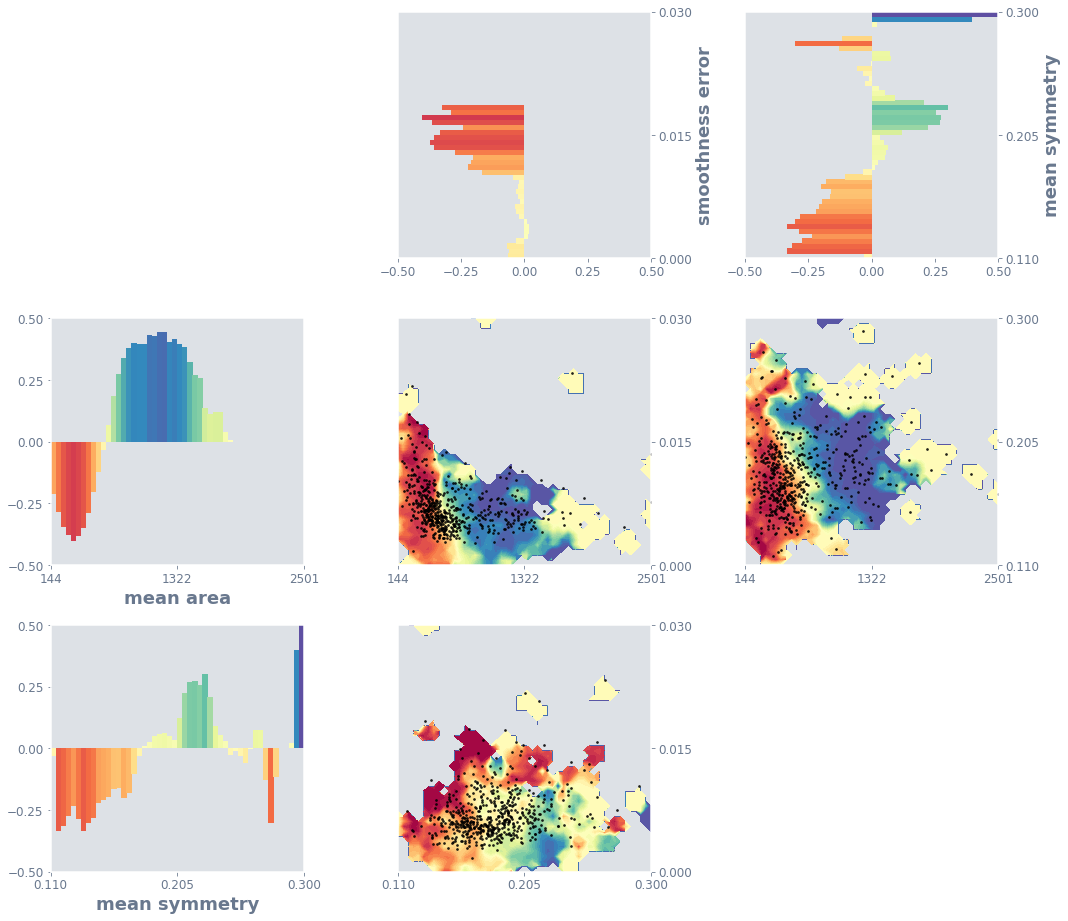
\includegraphics[width=\columnwidth]{img/rf_ocsvm_matrix.png}
\caption{RF with OCSVM interpolation. Blue indicates model certainty of benality, yellow of uncertainty, and red of malignancy. Lack of contour indicates a prediction outside the sample space. The bottom and right axis are the single dimension decomposition, while the middle countours represent the density of the cross dimensional decomposition. In the single dimension estimates, the resulting value is shifted down by 0.5 to create a flat midpoint for the bars.}
\label{fig:rf-ocsvm-matrix}
\end{figure}

\subsection{Neural Network and OCSVM Interpolation}

A 3 layer feed forward Neural Network (NN) was used; an input, a hidden layer where tanh is applied, and an output layer. Softmax is applied when making predictions, and the final certainty of the prediction is calculated by calculating the proportion of the largest weighted class out of all weightings. The NN was trained over 50,000 epochs and achieved an F1 score of 0.961, slightly worse than the RF. The NN was more binary with its predictions, 

\begin{figure}
\centering
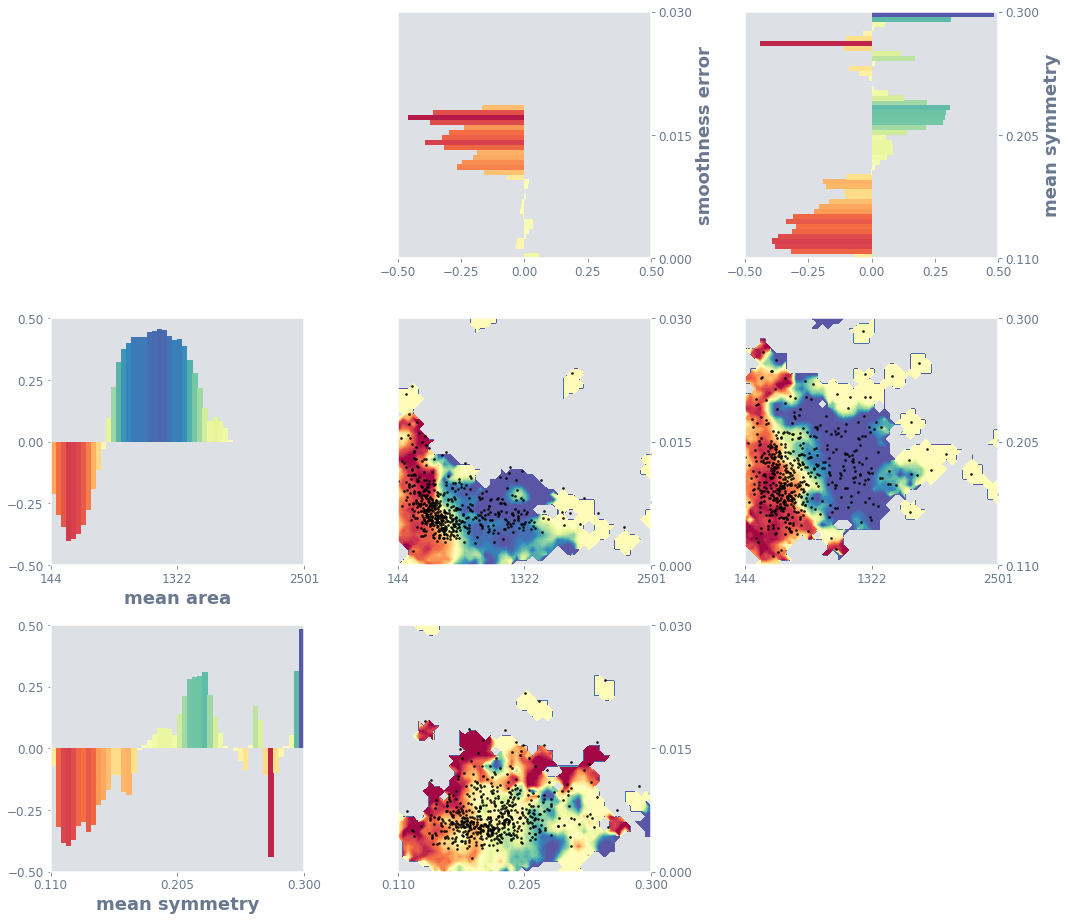
\includegraphics[width=\columnwidth]{img/nn_ocsvm_matrix.png}
\caption{NN with OCSVM interpolation.}
\label{fig:rf-ocsvm-matrix}
\end{figure}

\subsection{Analysis of Discrepancy Between RF and NN}

There is very little discrepancy between the two model, both of which have similar predictive success. However, random forests are widely regarded as more interpretable than neural networks []. The similarity of the two resultant visualizations is strong proof of the positive effect of LDR on model interpretability. The larger extreme value patches in the NN multi dimensional space are caused by the prediction density function interpreted by the final regression SVM being more steep to to the more binary classification of the SVM. This can be seen in the scatter plots of prediction certainties of the RF \ref{fig:rf-ocsvm-mean-symmetry-scatter} compared to the NN \ref{fig:nn-ocsvm-mean-symmetry-scatter}.

\begin{figure}
\centering
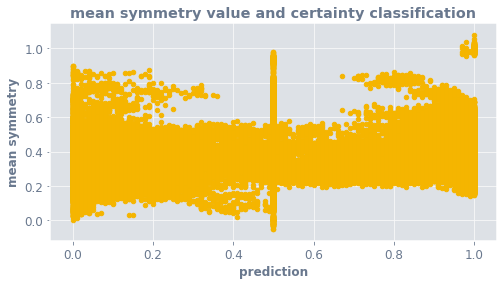
\includegraphics[width=\columnwidth]{img/rf_ocsvm_mean_symmetry.png}
\caption{RF prediction certainty scatter plot of mean symmetry.}
\label{fig:nn-ocsvm-mean-symmetry-scatter}
\end{figure}

\begin{figure}
\centering
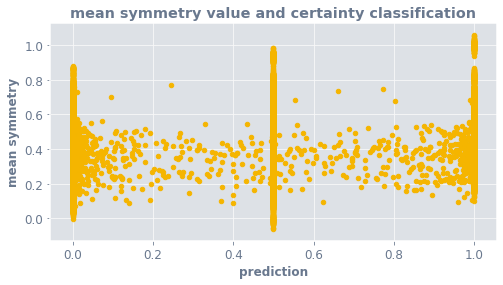
\includegraphics[width=\columnwidth]{img/nn_ocsvm_mean_symmetry.png}
\caption{NN prediction certainty scatter plot of mean symmetry.}
\label{fig:nn-ocsvm-mean-symmetry-scatter}
\end{figure}

\section{Regression Example}

A similar method as with the classification was applied to the Boston House Price dataset []. This dataset has 14 dimensions, where the target is to predict the house price based off of quantitative factors such as proximity to radial highways, age and per Nitric Oxide concentration. Some interesting relations made immediately available from the LDR, shown in figure \ref{fig:reg-rf-ocsvm-matrix}, are

\begin{figure}
\centering
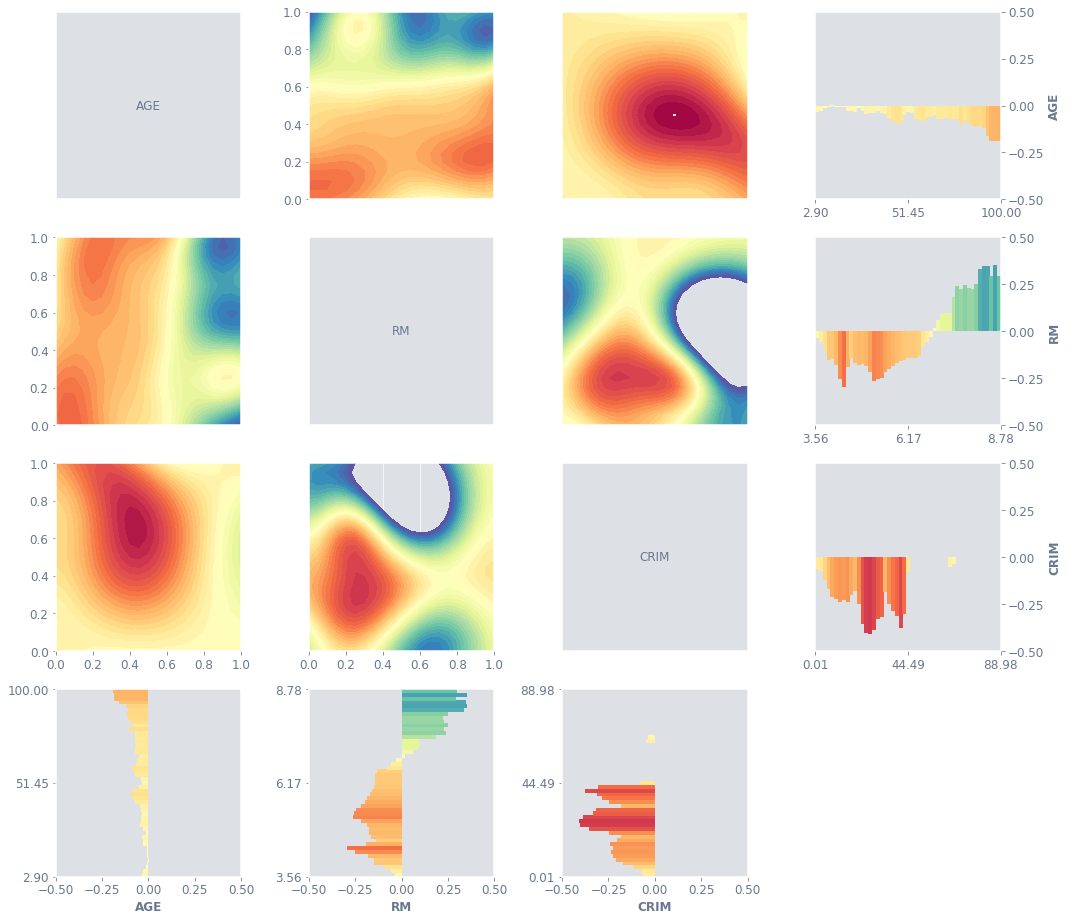
\includegraphics[width=\columnwidth]{img/reg_rf_ocsvm_matrix.png}
\caption{Regression RF with OCSVM interpolation. AGE is the age of the house, RM the number of rooms, and CRIM the per capita crime rate per town.}
\label{fig:reg-rf-ocsvm-matrix}
\end{figure}

\begin{enumerate}
\item An increasing crime rate tends to correlated with houses being worth less. Above the median level of crime however, the model becomes unsure.
\item Crime only has a negative effect on house price.
\item Houses with fewer rooms but a lower level of crime are worth similar to those with a higher level of crime but more rooms. There are however not many houses in areas with high amounts of crime and lots of rooms.
\item The older the house, the less it tends to be worth.
\item For the most part, the age of the house and the number of rooms are uncorrelated.
\end{enumerate}

The process for an individual dimension can be seen in figure \ref{fig:reg-rf-ocsvm-rm}.

\begin{figure}
\centering
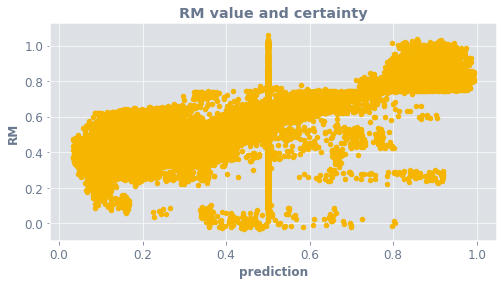
\includegraphics[width=\columnwidth]{img/reg_rf_ocsvm_rm.png}
\caption{RF prediction certainty of number of rooms.}
\label{fig:reg-rf-ocsvm-rm}
\end{figure}

\section{Mathematical Explanation}

Let $\Omega$ be the total sample space of input data. Let $X \in \Omega$ describe an input vector of data of length $n$, where each $x_i \in [0, 1]$ is the scaled value for feature $i$ in the vector.

$$X = \{x_1, x_2, \ldots, x_n\}$$

Let $Y$ be a single or multivariate output vector ($Y = y$ if single) where each $y_i$ is a predicted variable.

$$Y = \{y_1, y_2, \ldots, y_n\}$$

Let $s \in [0, 1]$ be a prediction of an outlier, s.t. 1 indicates an outlier and 0 not an outlier.

Let $m$ describe a model as a function s.t. $m(X) = Y$, and $o$ describe an outlier classifier function s.t. $o(X) = s$

$$m(X) = Y$$

$$o(X) = s$$

Let the outlier weighting and model prediction interpolation function $f$ be defined as

$$f(X) = (m(X) - 0.5) \times o(X) + 0.5$$

Let the resolution of a KDE bandwidth be $r$. The KDE function $g$ over a $n$ samples can therefore be defined as

$$g(X) = \frac{1}{nr} \sum^n_{i=1} K \frac{x - x_i)}{h}$$

which is effectively an implementation of the VEGAS algorithm for the Monte Carlo Integration function $I_\Omega$.

Let the set of points drawn from $\Omega$ be $Q$, where $q \in {i*r}^{1/r}_0$ while $x_i$ are drawn from $g$. $Q$ can therefore be described as

$$Q = {x_1, x_2, \ldots, q, \ldots, x_n}$$

One option for model certainty and outlier interpolation estimation is therefore given by

$$I_\Omega = \{\frac{1}{n} \sum^n_{i=1} f(Q(X))\}$$

While an alternative method is to use an SVM, or alternative predictive model, to model the function describing the dimensionality reduced space model certainty. Let this model be defined as $h$, resulting in

$$I_\Omega = h(Q(X))$$

\section{Conclusion}\label{Conclusion}

This method will require either formal proof of efficacy or significant demonstration of reliable practical use before it should be used in the field.

\printbibliography

\end{document}